\section{Wheel Brake System}
\label{sec:wbs}
To demonstrate the fault modeling capabilities of the Safety Annex we will use the Wheel Brake System (WBS) described in AIR6110~\cite{AIR6110}.  This system is a well-known example that has been used as a case study for safety analysis, formal verification, and contract based design~\cite{DBLP:conf/cav/BozzanoCPJKPRT15, 10.1007/978-3-319-11936-6-7, CAV2015:BoCiGrMa, Joshi05:SafeComp}. The preliminary work for the Safety Annex was based on a simple model of the WBS~\cite{Stewart17:IMBSA}. To demonstrate a more complex fault modeling process, we constructed a functionally and structurally equivalent AADL version of the more complex WBS NuSMV/xSAP models~\cite{DBLP:conf/cav/BozzanoCPJKPRT15}.    

\begin{figure}[htbp]
	\centering
	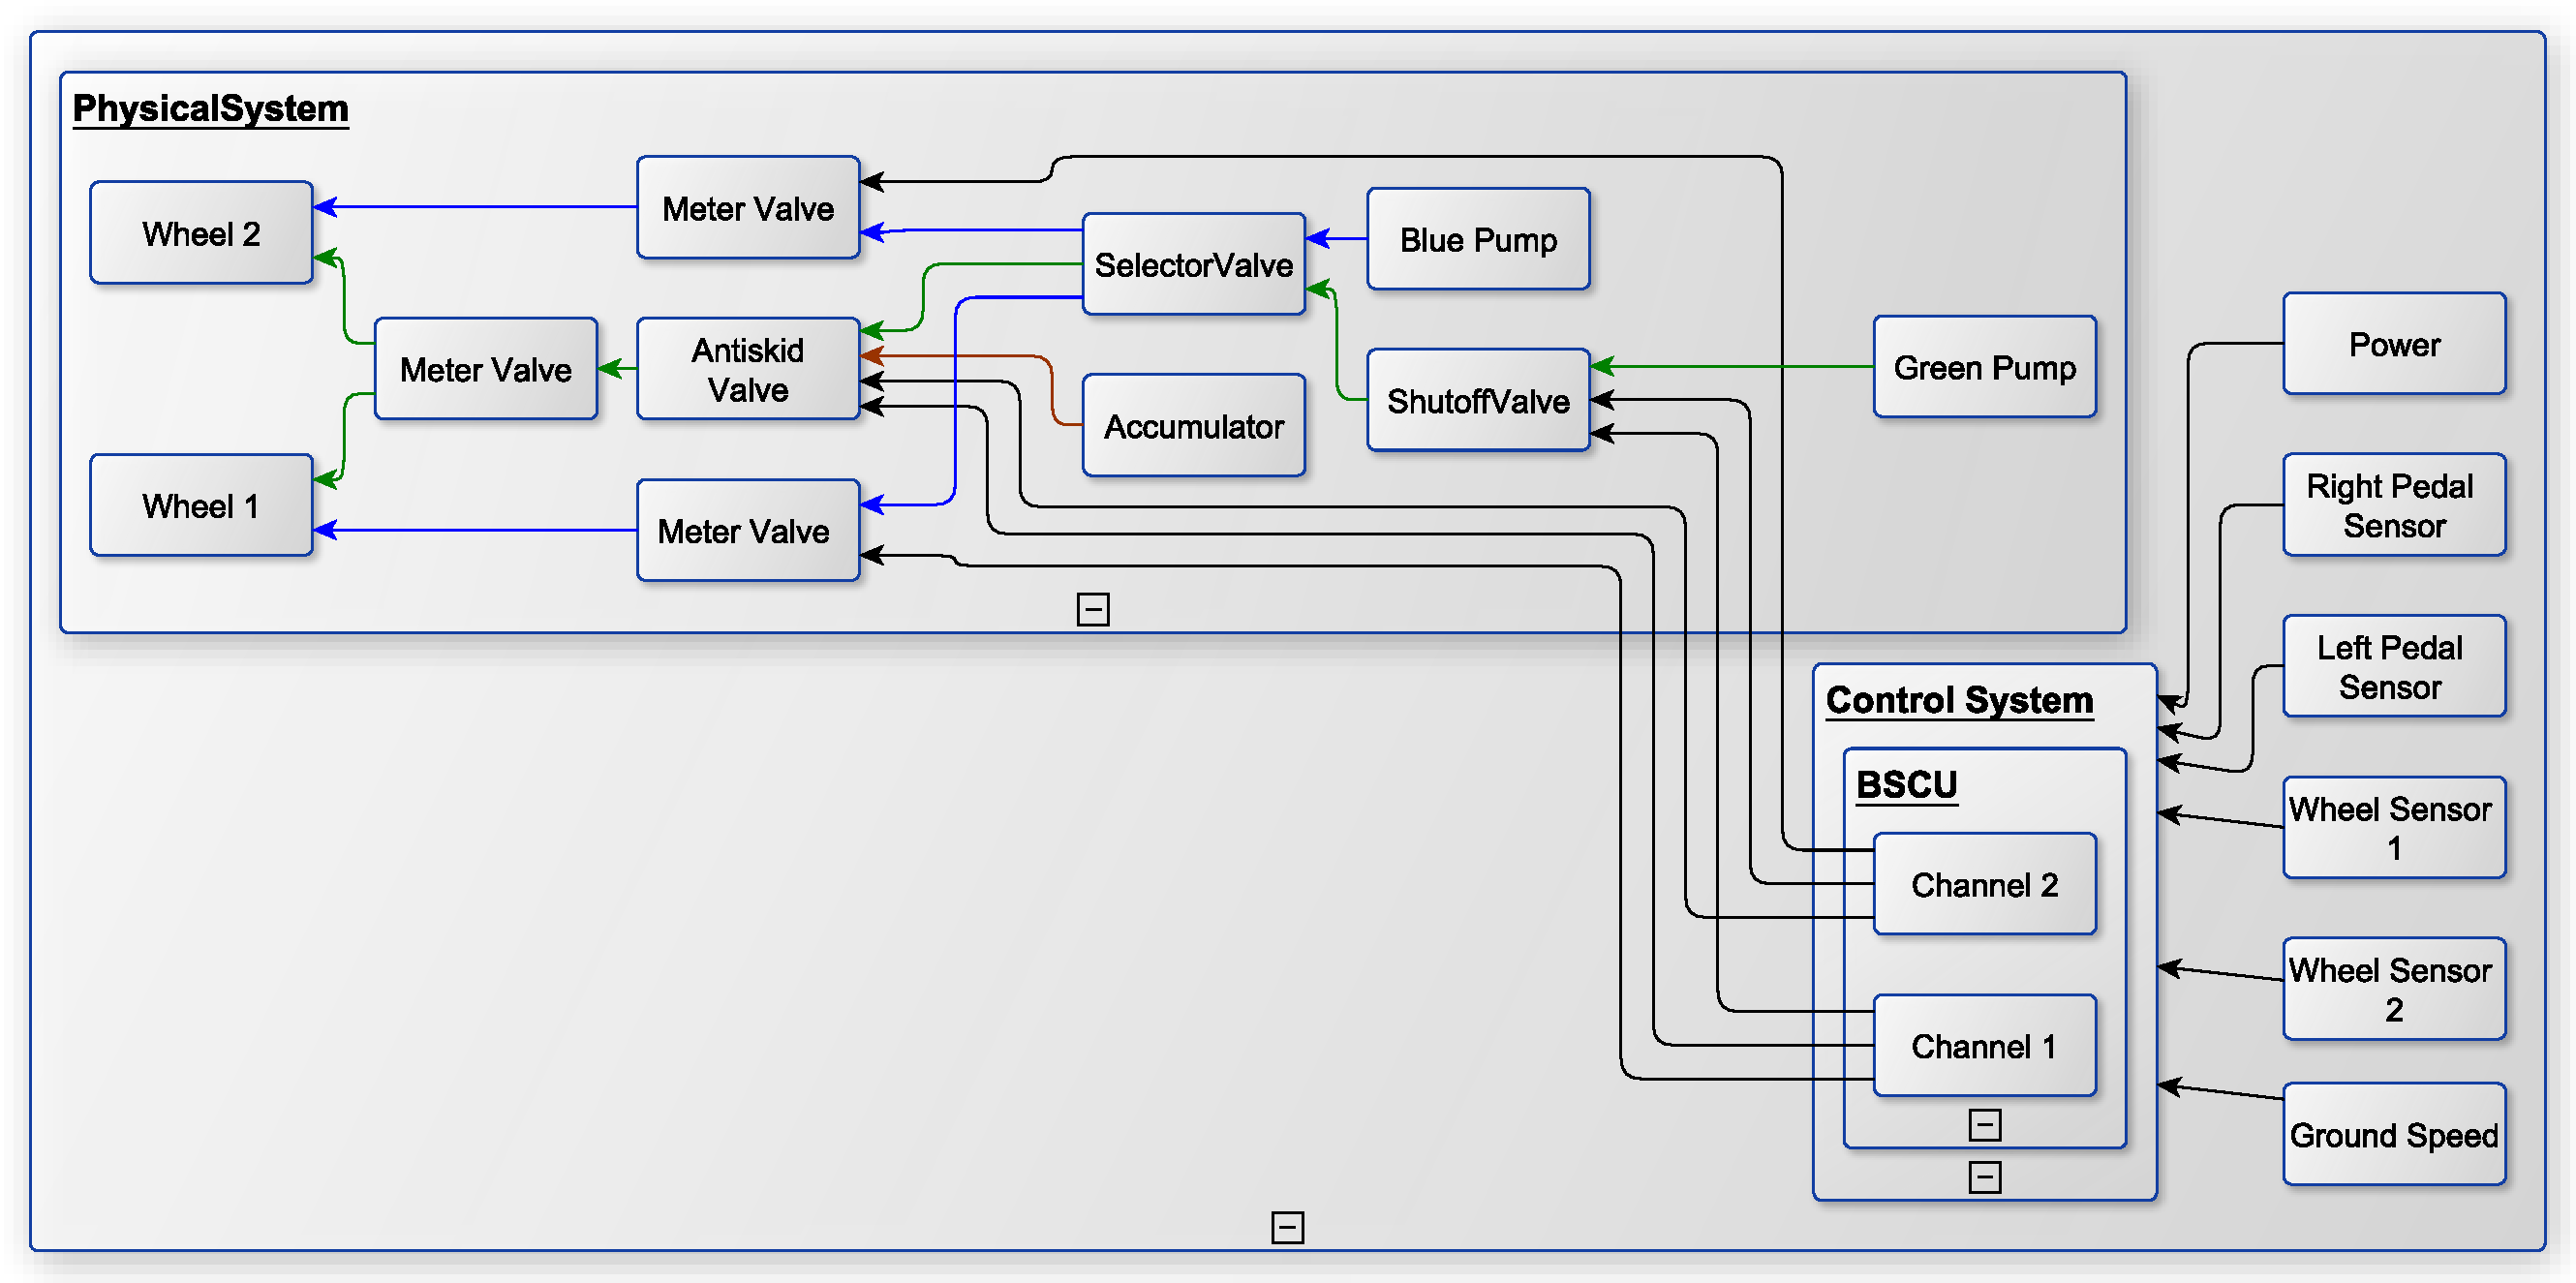
\includegraphics[trim=0 9 0 5,clip,width=\textwidth]{images/wbs_arch4_diagram.pdf}
	\caption{Simplified Two-Wheel WBS}
	\label{fig:wbs}
\end{figure} 

The WBS is composed of two main parts: the Line Replaceable Unit control system and the electro-mechanical physical system.
The control system electronically controls the physical system and contains a redundant
channel of the Braking System Control Unit (BSCU) in case a detectable fault occurs in the active channel.
The control system also commands antiskid braking. % in case of skidding on the ground. 
 The physical system consists of the hydraulic circuits running from hydraulic pumps to wheel brakes as well as valves that control the hydraulic fluid flow. This system provides braking force to each of the eight wheels of the aircraft. The wheels are all mechanically braked in pairs (one pair per landing gear). For simplicity, Figure~\ref{fig:wbs} displays only two of the eight wheels. 

There are three operating modes in the WBS model:

\begin{itemize}
	\renewcommand{\labelitemi}{\textbullet}
	\item In \textit{normal} mode, the system is operated by a \textit{green} hydraulic pump and one meter valve per each of the eight wheels. Each of the meter valves are controlled through electronic commands coming from the active channel of the BSCU. These signals provide braking and antiskid commands for each wheel. The braking command is determined through a sensor on the pedal and the antiskid command is determined by the \textit{Wheel Sensors}. 
	\item In \textit{alternate} mode, the system is operated by a \textit{blue} hydraulic pump, four meter valves, and four antiskid shutoff valves, one for each landing gear. The meter valves are mechanically commanded through the pilot pedal corresponding to each landing gear. If the selector detects lack of pressure in the green circuit, it switches to the blue circuit. 
	\item \textit{Emergency} mode is entered if the \textit{blue} hydraulic pump fails. The accumulator pressure vessel has a reserve of pressurized hydraulic fluid and will supply this to the blue circuit in emergency mode. 
\end{itemize}

The WBS architecture model in AADL contains 30 different kinds of components, 169 component instances, and a model depth of 5 hierarchical levels. 

The behavioral model is encoded using the AGREE annex and the behavior is based on descriptions found in AIR6110. The top level system properties are given by the requirements and safety objectives in AIR6110. All of the subcomponent contracts support these system safety objectives through the use of assumptions on component input and guarantees on the output. 

An example system safety property is to ensure that there is no inadvertent braking of any of the wheels. This is based on a failure condition described in AIR6110 is \textit{Inadvertent wheel braking on one wheel during takeoff shall be less than $10^{-9}$ per takeoff}. 
Inadvertent braking means that braking force is applied at the wheel but the pilot has not pressed the brake pedal.  In addition, the inadvertent braking requires that power and hydraulic pressure are both present, the plane is not stopped, and the wheel is rolling (not skidding). Figure \ref{fig:inadvertent_braking} shows the AGREE specification of this property. If power and hydraulic pressure are supplied and the pedal is not pressed, that implies that the wheel isn't rolling, speed is zero, or there is no braking force supplied at the wheel.

\begin{figure}[htbp]
	%\vspace{-0.2in}
	\begin{center}
		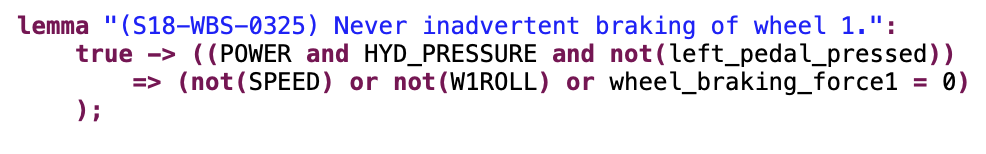
\includegraphics[width=.9\textwidth]{images/inadvBraking.png}
	\end{center}
	\vspace{-0.3in}
	\caption{Safety Property: Inadvertent Braking}
	\label{fig:inadvertent_braking}
	%\vspace{-0.2in}
\end{figure}

\subsection{Nominal Model Analysis}
Before performing fault analysis, users should first check that the safety properties are satisfied by the nominal design model. This analysis can be performed monolithically or compositionally in AGREE. Using monolithic analysis, the contracts at the lower levels of the architecture are flattened and used in the proof of the top level safety properties of the system. Compositional analysis, on the other hand, will perform the proof layer by layer top down, essentially breaking the larger proof into subsets of smaller problems. For a more comprehensive description of these types of proofs and analyses, see additional publications related to AGREE \cite{cofer2012compositional,QFCS15:backes} and we refer you to Section~\ref{sec:concepts}.

The WBS has a total of 13 safety properties at the top level that are supported by subcomponent assumptions and guarantees. These are shown in Table \ref{tab:safetyProperties}. Given that there are 8 wheels, contract S18-WBS-0325-wheelX is repeated 8 times, one for each wheel. The behavioral model in total consists of over 440 assumptions and guarantees after instantiation.

\begin{table}[htbp]
\begin{center}
\begin{tabular}{@{}ll}
\toprule
\textbf{S18-WBS-R-0321} \\Loss of all wheel braking during landing shall have a probability of occurrence less than \\$5.0 \times 10^{-7}$ per flight.                                    \\ \midrule 
\textbf{S18-WBS-R/L-0322}  \\ Asymmetrical loss of wheel braking (Left/Right) shall have a probability of occurrence\\less than $5.0 \times 10^{-7}$ per flight. \\ \midrule
\textbf{S18-WBS-0323} \\ Inadvertent braking with all wheels locked shall have a probability of occurrence less \\than $10^{-9}$ per takeoff.                                                                                                                                                                                                               \\ \midrule
\textbf{S18-WBS-0324}  \\ Inadvertent braking with all wheels shall have a probability of occurrence less than $10^{-9}$ \\per takeoff.                                                                                                            \\ \midrule
\textbf{S18-WBS-0325-wheelX} \\ Inadvertent braking of wheel X shall have a probability of occurrence less than $10^{-9}$ \\per takeoff.                                                                                                                                                                                                                           \\ \bottomrule
\end{tabular}
\caption{Safety Properties of the WBS}
\label{tab:safetyProperties}
\end{center} 
\end{table} 

The analysis results are shown in Figure~\ref{fig:analysisResults}. 

\begin{figure}[htbp]
	%\vspace{-0.2in}
	\begin{center}
		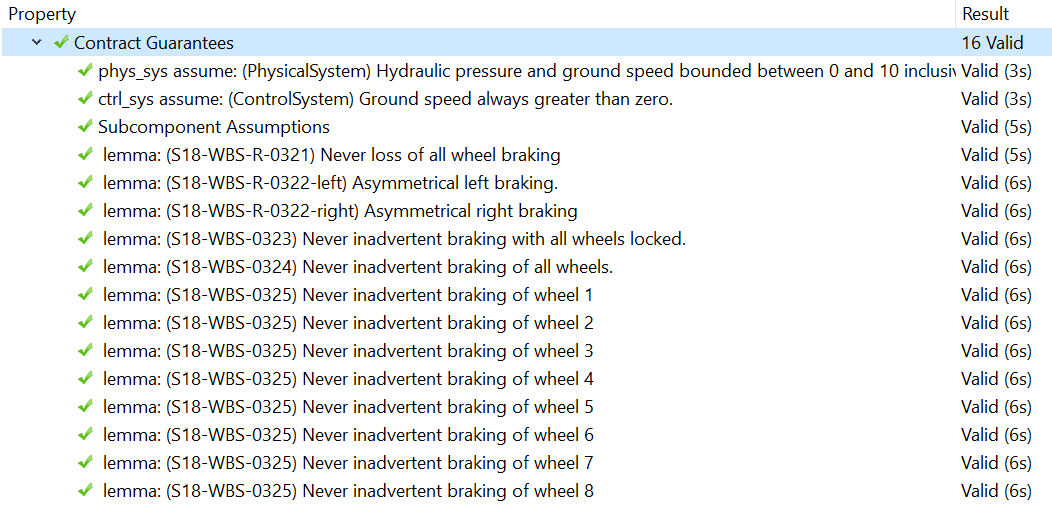
\includegraphics[width=.9\textwidth]{images/nominalModelResults.png}
	\end{center}
	\vspace{-0.3in}
	\caption{Nominal model analysis results for WBS}
	\label{fig:analysisResults}
	%\vspace{-0.2in}
\end{figure}

The lemmas are the specifications of all top level safety properties in the model. The results show that the model supports the specifications and a proof is found for each lemma. The child component contracts are used to prove the validity of the safety properties.

\subsection{Fault Model Analysis}
There are two main options for fault model analysis using the Safety Annex. The first option injects faults into the Lustre program based on the restrictions placed through the fault hypothesis. The bounded model checker engine used in JKind will find counterexamples to an invalid property. These counterexamples are returned to the user and include a trace of the system execution that causes the violation. This includes any active faults that were part of that violation. The second option is used to generate minimal cut sets for the model. The fault activation literals and supporting guarantees are added to the MIVC algorithm elements as described in Sections~\ref{sec:formalization} and \ref{sec:impl}, the algorithm generating the cut sets is run (Section~\ref{sec:impl}), and the results are displayed to the user. 

\subsubsection{Verification in the Presence of Faults: Max \textit{n} Analysis}
Using a max number of faults for the hypothesis, the user can constrain the number of simultaneously active faults in the model. The faults are added to the AGREE model for the verification. Given the constraint on the number of possible simultaneously active faults, the model checker attempts to prove the top level properties given these constraints. If this cannot be done, the counterexample provided will show which of the faults ($n$ or less) are active and which contracts are violated. More detail on verification of fault models can be found in Section~\ref{sec:analysisResults}. 

The WBS was verified in the presence of faults given a \texttt{max 1 fault} hypothesis using compositional analysis. The time for complete model analysis was approximately 9 minutes, but a counterexample for certain top level properties took only around 20 seconds. (Recall that when using compositional verification in the presence of faults, that hypothesis applies to each layer separately -- the results are not rolled up as in the compositional generation of minimal cut sets. The counterexample given in this analysis pertains only to faults and contracts \textit{in a given layer}, and the timing of the counterexample reflects this single layer analysis result.) 

The verification in the presence of faults with \texttt{max 1 fault} hypothesis statement provided a counterexample to the property {\em S18-WBS-0325: never inadvertent braking of wheel i}, for $i = 1, \dots 8$. This property is given in Figure~\ref{fig:inadvertent_braking}. The intuition behind the failure is that the pedal was not pressed, the sensor failed and sent a signal stating that the pedal was pressed, braking was commanded through the digital components, and brake pressure was supplied at the wheel. The failed sensor was a single point of failure with regard to all of the inadvertent braking properties. Later in this section we look at the sensor on the pedal position in closer detail from the lens of architectural design changes guided by the analysis results. 

\subsubsection{Verification in the Presence of Faults: Probabilistic Analysis} 
Given a probabilistic fault hypothesis, this corresponds to performing analysis with the combinations of faults whose occurrence probability is less than the probability threshold. This is done by inserting assertions that allow those combinations in the Lustre code. If the model checker proves that the safety properties can be violated with any of those combinations, one of such combination will be shown in the counterexample. Probabilistic analysis done in this way must utilize the monolithic AGREE option. 

Recall that when using the \texttt{max 1 fault} hypothesis statement on the WBS, we found that the sensor was a single point of failure for multiple properties. The probability of this particular sensor failing is given in AIR6110~\cite{AIR6110} as $1.0 \times 10^{-2}$. The probabilistic hypothesis was set according to the thresholds given per property (see Table~\ref{tab:safetyProperties}) and the analysis was run monolithically on the WBS model. The total time {\em to generate a counterexample} for violated properties using a probabilistic hypothesis with monolithic analysis varied depending on the safety property; the range of times was between 15 seconds and 9 minutes\footnote{All following analyses were run on an Intel Core i7 with a 2.80GHz CPU and 16 GB RAM. }. 
The property that took the longest to generate a counterexample for was {\em S18-WBS-0323: inadvertent braking with all wheels locked shall have a probability of occurrence less than $1.0 \times 10^{-9}$ per takeoff.} The formula for this property references all 8 wheels and numerous subcomponents, most of which have faults associated with them. The low probability threshold combined with the formula complexity and the exponential increase in fault combinations likely served to make this the longest time in counterexample generation. For a full discussion on use of probabilistic thresholds in compositional analysis, see Section~\ref{sec:prob_generate}.

\subsubsection{Generate Minimal Cut Sets: Max \textit{n} Analysis}
\label{sec:maxN_generate}
As described in Section~\ref{sec:impl}, we use the \aivcalg algorithm to provide a full enumeration of all minimal set of model elements necessary for the proof of each top-level safety property in the model, and then transform all MIVCs into all minimal cut sets. In max $n$ analysis, the minimal cut sets are pruned to include only those with at cardinality less than or equal to the number $n$ specified in the fault hypothesis.

Generate minimal cut set analysis was performed on the Wheel Brake System and results are shown in Table~\ref{tab:wbs_maxN_results1}. The label across the top row refers to the cardinality (\textit{n}) and the corresponding column shows how many cut sets are generated of that cardinality. When the analysis is run, the user specifies the value \textit{n}. This gives cut sets of cardinality less than or equal to \textit{n}. Table~\ref{tab:wbs_maxN_results1} shows the total number of cut sets of cardinality \textit{n}. The total number of cut sets computed at the given threshold is the sum across a row. (For the full text of the properties, see Table~\ref{tab:safetyProperties}.) 


\begin{table}[htbp]
\begin{center}
    \begin{tabular}{ | l | l | l | l | l | l |}
    \hline
    \textbf{Property} & $\bm{n = 1}$ & $\bm{n = 2}$ & $\bm{n = 3}$ & $\bm{n = 4}$ 
		& $\bm{n = 5}$    \\ \hline \hline
    0321 & 6 & 0 & 0 & 256 & 57,600   \\ \hline
    0322-R & 18 & 0 & 0 & 0 & 0  \\ \hline
    0322-L & 18 & 0 & 0 & 0 & 0  \\ \hline
    0323 & 2 & 0 & 0 & 0 & 0  \\ \hline
    0324 & 8 & 3,665 & 28,694 & 883,981 & - \\ \hline
    0325-WX & 18 & 0 & 0 &0 &0 \\ \hline
    \end{tabular}
    \caption{WBS Minimal Cut Set Results for Max \textit{n} Hypothesis}
    \label{tab:wbs_maxN_results1}
    \end{center}
\end{table}


For property 3024, the number of cut sets increases as the cardinality of allowable cut sets grows. Intuitively, this can be understood as simple combinations of faults that can violate the hazard; if more things go wrong in a system at the same time, the more likely this property will be violated. Property S18-WBS-0324 with a max fault hypothesis of 5 was unable to finish due to an out of memory error. At the time that the error was thrown, the number of cut sets exceeded 1 million. In practice, it is not likely that an analyst will manually sift through a million or more cut sets, but rather will filter out the combinations that are sufficiently unlikely to occur. A probabilistic approach would be warranted in these situations. 

The next analysis shows the difference between the time it takes to generate all MIVCs and the time it takes to transform those MIVCs into minimal cut sets. Each column of Table~\ref{tab:wbs_mincut1} labeled with the value of \textit{n} gives the fault hypothesis threshold for that analysis run. For comparison with the number of minimal cut sets generated per property, we refer to Table~\ref{tab:wbs_maxN_results1}\footnote{The property S18-WBS-0325-WX is symmetric for all eight wheels. For readability, we only include wheel one verification timing results in Table~\ref{tab:wbs_mincut1}. Likewise for property 0322-L/R.}.
\begin{table}[htbp]
\begin{center}
    \begin{tabular}{ | l | l | l | l | l | l | l |}
    \hline
    \textbf{Property} &  MIVC Gen & $n=1$ & $n=2$ & $n=3$ & $n=4$ & $n=5$     \\ \hline \hline
    0321 & 396.417 & 5.913 & 5.468 & 5.61 & 5.636 & 11.925  \\ \hline
    0322-L  & 407.078 & 5.931 & 5.435 & 5.302 & 5.268 & 5.243 \\ \hline
    0323 & 412.926 & 6.397 & 6.452 & 6.420  & 5.309 & 5.459\\ \hline
    0324 & 446.610 & 21.334 & 41.744 & 44.062 & 69.142 & -\\ \hline
    0325-W1 & 391.137 & 5.632 & 5.388 &5.359 &5.301 & 5.236 \\ \hline
    \end{tabular}
    \caption{WBS Analysis Time in Seconds}
    \label{tab:wbs_mincut1}
    \end{center}
\end{table}
The overall time of the algorithms used for minimal cut set generation is quite small compared to the nominal analysis and extended model analysis time. This is likely due to the thresholds used to prune the size of the cut sets computed. At each layer of analysis, pruning can take place that may shrink the problem space considerably. The greatest time recorded was for property S18-WBS-0324 at $n = 4$; the reason is clear when comparing this with Table~\ref{tab:wbs_maxN_results1}: the total number of minimal cut sets computed for this threshold is over 800,000.  

\subsubsection{Generate Minimal Cut Sets: Probabilistic Analysis}
\label{sec:prob_generate}
Both probabilistic analysis and max $n$ analysis use the same underlying minimal cut set generation algorithm, but in probabilistic analysis the minimal cut sets are pruned to include only those fault combinations whose probability of simultaneous occurrence exceed the given threshold in the hypothesis. 

The probabilistic analysis for the WBS was given a top level threshold per property as stated in AIR6110 and shown in Table~\ref{tab:safetyProperties}. The faults associated with various components were all given probability of occurrence according to the AIR6110 document~\cite{AIR6110}. The table shows the property name and associated probability. The generation of minimal cut sets provided all sets that violate that property whose combined probabilities (assuming independence) are greater than the threshold. The number of sets per cardinality are listed in the table. 

\begin{table}[htbp]
\begin{center}
    \begin{tabular}{ | l | l | l | l | l | l | l | }
    \hline
    \textbf{Property} & $n=1$ & $n=2$ & $n=3$ & $n=4$ 
		& $n=5$    \\ \hline \hline
    0321: $5.0 \times 10^{-7}$ & 6 & 0 & 0 & 0 & 0   \\ \hline
    0322-R: $5.0 \times 10^{-7}$ & 18 & 0 & 0 &0 &0   \\ \hline
    0322-L: $5.0 \times 10^{-7}$ & 18 & 0 & 0 & 0 & 0    \\ \hline
    0323: $1.0 \times 10^{-9}$ & 2 & 0 & 0 & 0 & 0    \\ \hline
    0324: $1.0 \times 10^{-9}$ & 8 & 256 & 0 & 0 & 0   \\ \hline
    0325-W1: $1.0 \times 10^{-9}$ & 8 & 0 & 0 &0 &0    \\ \hline
    \end{tabular}
    \caption{WBS Minimal Cut Set Results for Probabilistic Hypotheses}
    \label{tab:wbs_prob_results}
    \end{center}
\end{table}

As shown in Table~\ref{tab:wbs_prob_results}, the number of allowable combinations drops considerably when given probabilistic threshold as compared to just fault combinations of certain cardinalities. For example, one contract (0324: inadvertent wheel braking of all wheels) had over a million minimal cut sets produced when looking at it in terms of max N analysis, but after taking probabilities into account, it is seen in Table~\ref{tab:wbs_prob_results} that the likely contributors to a hazard are minimal cut sets of cardinality one or two. The probabilistic analysis eliminated many thousands of cut sets from consideration. The total computation time for these runs is given in Table~\ref{tab:analysisTimeWBSProb}.


\begin{table}[htbp]
\begin{center}
    \begin{tabular}{ | l | l | l | l | l | l | l | }
    \hline
    \textbf{Property} & Total Analysis Time   \\ \hline \hline
    R-0321: $5.0 \times 10^{-7}$ & 433.144 sec  \\ \hline
    R-0322: $5.0 \times 10^{-7}$  & 431.954 sec  \\ \hline
    L-0322: $5.0 \times 10^{-7}$  & 429.081 sec    \\ \hline
    0323: $1.0 \times 10^{-9}$  & 571.216 sec    \\ \hline
    0324: $1.0 \times 10^{-9}$ & 589.07 sec   \\ \hline
    0325-W1: $1.0 \times 10^{-9}$ & 430.021 sec    \\ \hline
    \end{tabular}
    \caption{WBS Minimal Cut Set Time for Probabilistic Hypothesis}
    \label{tab:analysisTimeWBSProb}
    \end{center}
\end{table}


It is clear that the lower probabilistic threshold for properties 0323-0325-WX allowed more fault combinations to be possible which increased computation time. One must also recall property 0324 from the max \textit{n} analysis whose threshold of $n=4$ produced close to a million cut sets of various cardinalities. The pruning according to probabilities cut out many of these sets from consideration; they are sufficiently unlikely to occur together. 

\subsubsection{Display Minimal Cut Sets}
Results from minimal cut set analysis can be represented in one of the following forms. 
\begin{enumerate}
\item The minimal cut sets can be presented in text form with the total number per property, cardinality of each, and description strings showing the property and fault information. A sample of this output is shown in Figure~\ref{fig:detailedMCS}. 
\begin{figure}[htbp]
	\hspace*{-2cm}
	\vspace{-0.1in} 
	\begin{center}
		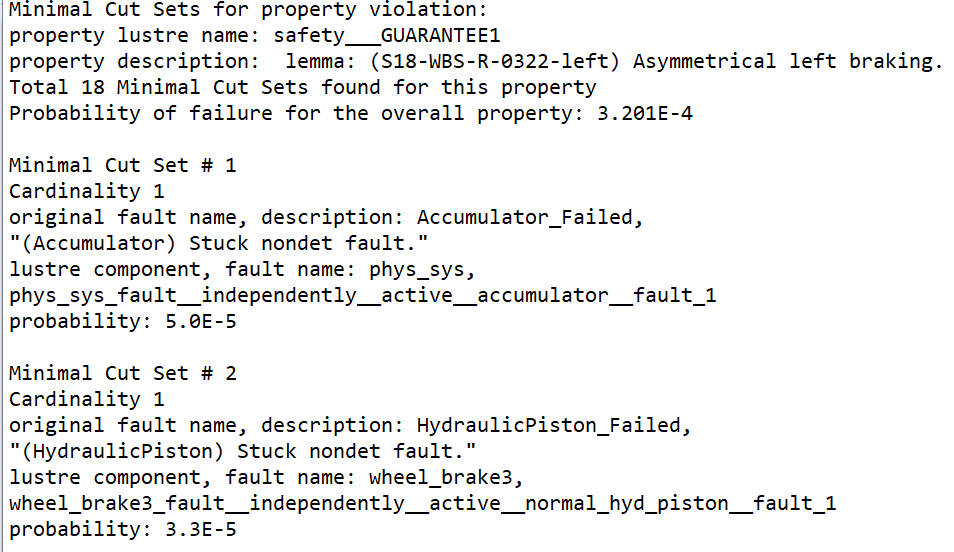
\includegraphics[scale=0.7]{images/mcs_detailed.png}
	\caption{Detailed Output of Minimal Cut Sets}
		\label{fig:detailedMCS}
	\end{center}
\end{figure}

\item The minimal cut set information can be presented in tally form. This does not contain the fault information in detail, but instead gives only the tally of cut sets per property. This is useful in large models with many cut sets as it reduces the size of the text file. An example of this output type is seen in Figure~\ref{fig:tallyMCS}.
\begin{figure}[htbp]
	\hspace*{-2cm}
	\vspace{-0.1in} 
	\begin{center}
		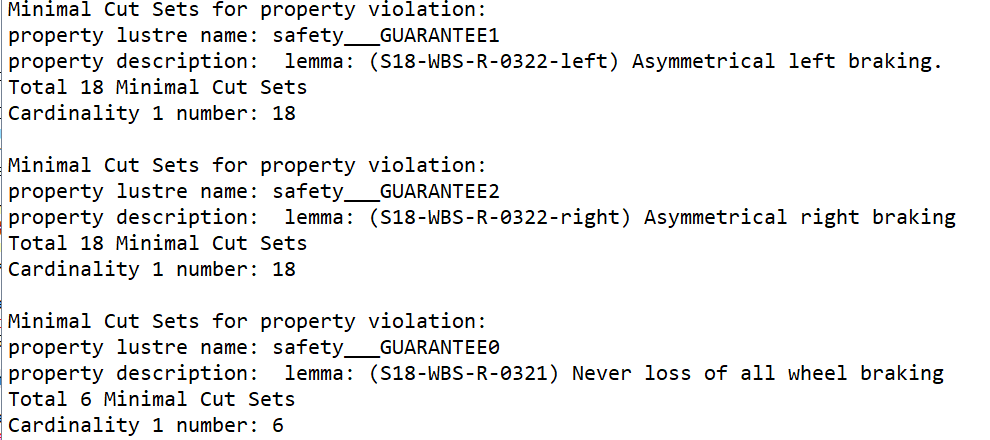
\includegraphics[scale=0.7]{images/mcs_tally.png}
	\caption{Tally Output of Minimal Cut Sets}
		\label{fig:tallyMCS}
	\end{center}
\end{figure}

\end{enumerate}

\subsubsection{Use of Analysis Results to Drive Design Change}
\label{sec:designChange}
We use a single top level requirement of the WBS: {\em S18-WBS-0323: inadvertent braking with all wheels locked shall occur with probability less than $10^{-9}$} to illustrate how the safety annex can be used to detect design flaws and how faults can affect the behavior of the system. 

Upon running max $n$ compositional fault analysis with $n = 1$, a pedal sensor fault was shown to be a single point of failure for the inadvertent braking properties. 
\begin{figure}[htbp]
	%\vspace{-0.2in}
	\begin{center}
		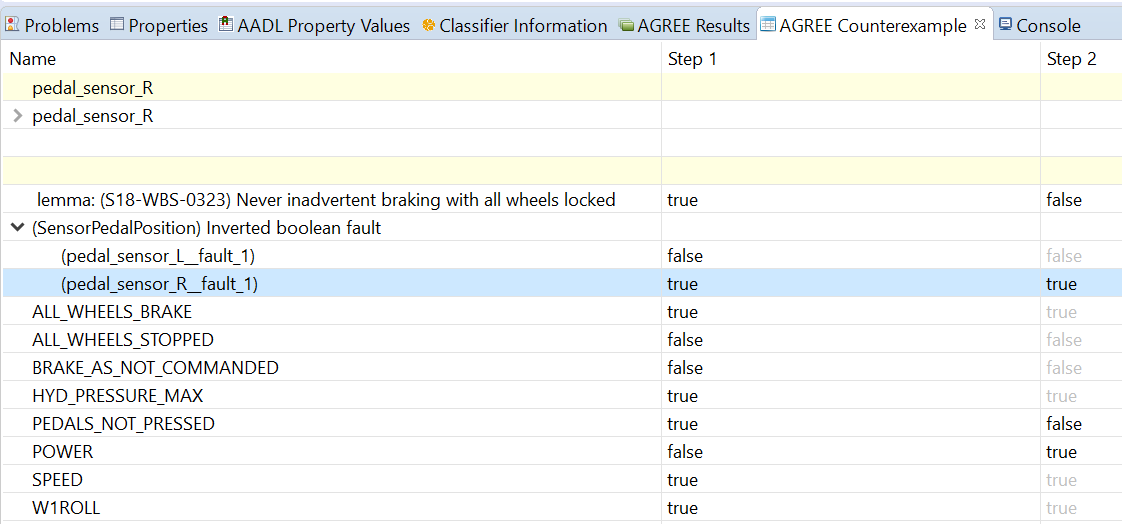
\includegraphics[width=0.8\textwidth]{images/counterexample.png}
	\end{center}
	\vspace{-0.3in}
	\caption{Counterexample for Inadvertent Braking}
	\label{fig:counterexample}
	%\vspace{-0.2in}
\end{figure} 
A counterexample is shown in Figure \ref{fig:counterexample} showing the active fault on the pedal sensor. Depending on the goals of the system, the architecture currently modeled, and the mitigation strategies that are desired, various strategies are possible to mitigate the problem.

\begin{itemize}
\item Possible mitigation strategy 1: Monitor system can be added for the sensor: A monitor sub-component can be modeled in which it accesses the mechanical pedal as well as the signal from the sensor. If the monitor finds discrepancies between these values, it can send an indication of an invalid sensor value to the top level of the system. In terms of the modeling, this would require a change to the behavioral contracts that use the sensor value. This validity would be taken into account through the means of $valid \land pedal\_sensor\_value$. 
%In the real system however, this mitigation would need to be taken into account. Whether this is a flag to the pilot who can then override the electrical system and switch to a different mode or perform some other action to mitigate the failed sensor must be discussed and implemented. 

\item Possible mitigation strategy 2: Redundancy can be added to the sensor: A sensor subsystem can be modeled which contains 3 or more sensors. The overall output from the sensor system may utilize a voting scheme to determine validity of sensor reading. There are multiple voting schemes that are possible, one of which is a majority voting (e.g., one sensor fails, the other two take a majority vote and the correct value is passed). 
When three sensors are present, this mitigates the single point of failure problem. New behavioral contracts are added to the sensor system to model the behavior of redundancy and voting. 
\end{itemize}
\begin{figure}[htbp]
	%\vspace{-0.2in}
	\begin{center}
		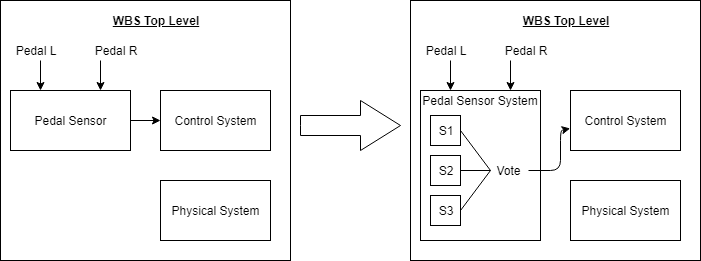
\includegraphics[width=0.7\textwidth]{images/sensorsystem.png}
	\end{center}
	\vspace{-0.3in}
	\caption{Architectural Changes for Fault Mitigation}
	\label{fig:sensorsystem}
	%\vspace{-0.2in}
\end{figure}
In the case of the pedal sensor in the WBS, the latter of the two strategies outlined above was implemented. A sensor system was added to the model which held three pedal sensors. The output of this subsystem was constrained using a majority voting scheme. Upon subsequent runs of the analysis (regardless which type of run was used), resilience was confirmed in the system regarding the failure of a single pedal sensor. Figure \ref{fig:sensorsystem} outlines the architectural changes that were made in the model.

As can be seen through this single example, a system such as the WBS would benefit from many iterations of this process. Furthermore, if the model is changed even slightly on the system development side, it would automatically be seen from the safety analysis perspective and any negative outcomes would be shown upon subsequent analysis runs. This effectively eliminates any miscommunications between the system development and analysis teams and creates a new safeguard regarding model changes. 

For more information on types of fault models that can be created as well as details on analysis results, see the users guide located in the GitHub repository \cite{SAGithub}. This repository also contains all models used in this project. 